CSCS is deploying logically isolated, versatile software-defined clusters (vClusters)\cite{vClusters2023} on the \crayex system Alps, to provide services to a wider range of user domains, each with their own software, security, reliability and scaling requirements.
The vClusters can be customized for each target use case, as an alternative to one large system that offers a ``one size fits all'' programming environment, storage and job scheduler configuration.

CSCS aims to reduce the complexity of the software installed on each vCluster through tailored user environments (uenv's).
These environments will provide the smallest possible set of compilers, libraries and tools optimized for vCluster's requirements, node architecture and the Slingshot 11 interconnect.
One obvious use case is for single purpose clusters, e.g., the production cluster of the Swiss weather service.
Alternatively, multiple use-case specific environments can be provided on general-purpose HPC vClusters, and loaded according to a user's individual needs.

This approach is at odds with the widely-adopted method to provide software on \crayex systems: installing the Cray Programming Environment (CPE), and building use-case specific software not provided by CPE on a shared file system, as illustrated in~\fig{fig:stacks}(a).
The CPE provides a wide range of software -- compilers, scientific libraries, communication libraries, debuggers, profiling tools, etc. -- all optimised for the node and network architecture of the system.
Furthemore, Cray continues to evolve and expand the CPE in response to changing requirements, for example adding software packages for ML/AI, with quarterly releases to address bugs, improve performance and add features.
Indeed, CSCS currently delivers such a one-size-fits-all environment, similarly to other HPC sites, using EasyBuild to provide additional software built and maintained by CSCS~\cite{forai:cug16}.

\begin{figure*}[htp!]
    \begin{center}
        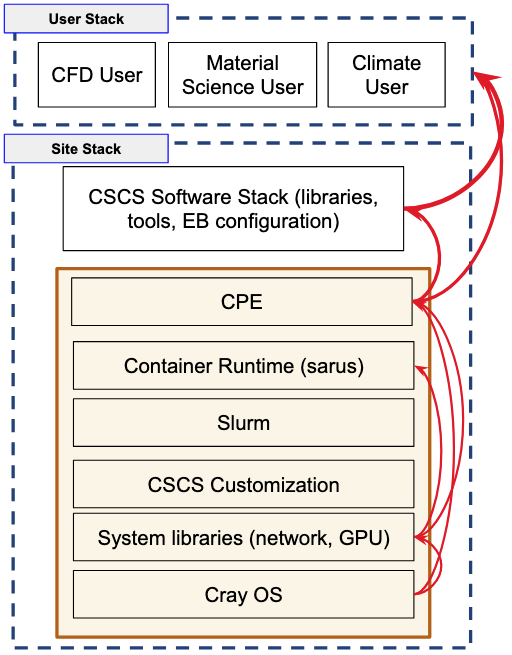
\includegraphics[width=0.35\textwidth]{./images/stack-old.png}
        \hspace{2.5cm}
        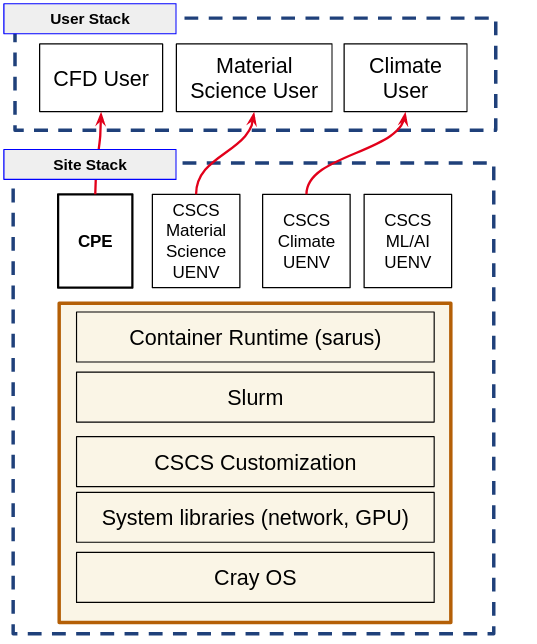
\includegraphics[width=0.35\textwidth]{./images/stack-new.png}
        \\
        \textbf{(a)} \hspace{9cm} \textbf{(b)}\\
    \end{center}
    \caption{
        \textbf{(a)}:
        The ``standard'' HPE-EX software stack, with the Cray OS, drivers, CPE and site-specific software in the system image, site-provided software installed on a shared file system. 
        User-installed software depends on the software layers underneath.
        The red arrows indicate where changes to one layer have a knock on effect on other software layers, requiring rebuilds or reconfiguration.\newline
        \textbf{(b)}:
        The Alps software stack with the programming environment moved out of the base image.
        Multiple programming environments can be deployed on top of this architecture. The CPE, and alternative PEs discussed in~\sect{sec:spack-stacks}, are mounted at runtime in a new mount namespace by users.
    }
    \label{fig:stacks}
\end{figure*}

However, while the CPE is a good general purpose environment for users, using it as a layer in HPC software stacks conflicts with our aim of reducing the complexity of software stacks.
In particular, two issues arise:
\begin{itemize}
    \item No single use-case or domain will use more than a small subset of the features provided by the CPE;
    \item Due to the CPE's quarterly cycle, the lead time between identifying an issue and a fix available and tested on site can be expected to be in the order of 3-6 months;
\end{itemize}
By striking a balance between long term stability and providing up-to-date software versions, CPE cannot fully satisfy use cases that only require either stability or timely fixes.

The work presented in this paper uses \spack and SquashFS images to build and deploy software stacks on top of a simplified base image that provides only the necessary vendor-specific libraries, for example libfabric, as illustrated in \fig{fig:stacks}(b).
Such a base image changes less frequently than CPE, reducing the need to rebuild software stacks with each CPE update and reducing system dependencies that could require intervention.

The result is compact, testable, reproducible and optimized software environments based on a descriptive recipe that can be updated independently of the CPE release cycle.

%\begin{enumerate}
%    \item long term stability -- software stack configuration can be maintained for longer
%    \begin{itemize}
%        \item requirement: reproducible builds
%        \item requirement: concise descriptive  recipes
%        \item requirement: minimise system requirements to only the bare minimum (no CPE)
%    \end{itemize}
%    \item rolling releases and fast fixes -- be able to rebuild and reconfigure at any point
%    \item provide use-case or application specific environments (only provide the required minimum)
%    \begin{itemize}
%        \item requirement: versioning of environments
%        \item requirement: fast deployment
%    \end{itemize}
%    \item deliver a satisfying user experience
%    \begin{itemize}
%        \item building and configuring software is fast and consistent (not dependent on file system performance).
%        \item compatibility with module, spack, python venv workflows.
%    \end{itemize}
%\end{enumerate}


%%% Local Variables:
%%% TeX-master: "paper"
%%% End:
